\section{Astrophysical Models}\label{sec:models}


%==============================================================================
\subsection{Basic Assumptions}\label{sec:basic}

We will assume that the mass and distance to \sgra is
\begin{eqnarray}
\label{eq:mass}
  \mbh &= (4.14 \pm 0.014) \times 10^6 \msun,\\
  D    &= (8.127 \pm 0.023) \kpc
\end{eqnarray}
which is approximately the mean of values reported by \citet{2019Sci...365..664D} and
\citet{2019A&A...625L..10G}.

Throughout the paper we also assume that \sgra is a black hole so that the spacetime around it is described by the Kerr metric. The black hole dimensionless spin, $\abh$, is a free parameter with $-1 < \abh < 1$, where $\abh \equiv Jc/G\mbh^2$, where $J$, $G$, and $c$ are the black hole angular momentum, gravitational constant, and speed of light, respectively.  Following \citetalias{M87PaperV}, $\abh < 0$ indicates the angular momentum of the accretion flow and black hole are antiparallel (the accretion flow is ``retrograde'').

Using the above mass and distance, the implied characteristic length ${\mathcal L} \equiv G M/c^2 = 6.1 \times 10^{11}\cm$, characteristic time ${\mathcal T} \equiv G M/c^3 = 20.5 \sec$, and angular scale ${\mathcal \theta_g} \equiv G\mbh/(c^2 D) = 5.03\uas$.  The expected diameter of the black hole shadow is $2\sqrt{27} G\mbh/(c^2 D) = (52.2 \pm 2.08) \uas $, where errorbars enclose uncertainty in the black hole spin and viewing angle (see e.g., \citealt{2020ApJ...896....7M}).

If the emitting plasma is ionized hydrogen (electron-proton plasma) then the Eddington luminosity is
$ L_\mathrm{Edd}
= 4\pi G\mbh c m_p/\sigma_{T}
= 5.2 \times 10^{44}\allowbreak \ergsps$.
The corresponding Eddington accretion rate is $ \dot\mbh_\mathrm{Edd} \equiv L_\mathrm{Edd}/(0.1 c^2)
= 5.8 \times 10^{24} \gm \sec^{-1}
= 0.09 \msun \yr^{-1}$ where nominal efficiency is 10\%
and the Eddington ratio:
$ L_\mathrm{bol}/L_\mathrm{Edd}
= 1.9 \times 10^{-10} (L_\mathrm{bol} /10^{35}) $ where $L_\mathrm{bol}$ is in $\erg\sec^{-1}$. In a quiescent, non-flaring state the bolometric luminosity of \sgra is $L_\mathrm{bol} \sim 10^{35}\erg\sec^{-1}$ resulting in an extremely small Eddington ratio. In what follows, we will assume that the radiative cooling of plasma around the black hole can be neglected and that model emission can be calculated in a post-processing step.

% below probably not necessary:
% \footnote{Translation of the source flux to luminosity is given by: $ \nu L_\nu
% = 4 \pi D^2 \nu F_\nu
% = 1.8 \times 10^{34} (D/8127 \pc)^2 \times\allowbreak
%   (\nu/230 \GHz)(F_\nu/{\rm Jy}) \erg \sec^{-1}$.}

%==============================================================================
\subsection{Estimate from One-Zone Model}

The development of complex models is guided by simple estimates. Following \citetalias{M87PaperV} we consider a one-zone model for \sgra. These results follow one-zone models developed in the literature over many decades (refs).

Our one-zone model is a uniform plasma sphere of radius $r = 5 \rg$ with uniform magnetic field oriented at $\pi/3$ to the line-of-sight. The magnetic pressure is given by $n_i k T_i + n_e k T_e = \beta B^2/(8\pi)$, where $T_i \equiv$ ion temperature, $T_e \equiv$ electron temperature, $\beta=1$, and $T_i = 3 T_e$.  We assume $\Theta_e \equiv  k T_e / m_e c^2 = 10$.

Using the thermal emissivity for synchrotron radiation $j_{\nu}$ (e.g., \citealt{2011ApJ...737...21L}) and assuming optically thin emission, the flux density in Jy is $F_\nu = (4/3)\pi r^3 j_\nu D^{-2} 10^{23}$.  Setting $F_\nu = 2.4$Jy (the average measured by ALMA during the 2017 campaign) yields a nonlinear equation for $n_e$ with solution
\begin{eqnarray}
\label{eq:onezone}
    n_e &\simeq& 1.1\times 10^6 \,\rm cm^{-3},\\
    B &\simeq& 30 \rm\, G.
\end{eqnarray}
(the synchrotron optical depth $\tau_S = r j_\nu/B_\nu \simeq 0.4$, so the optically thin approximation is marginal).
These values are consistent with $n_e$ and $B$ of a similar one-zone model fitted to archival Sgr~A* millimeter spectrum as reported in \citet{2019ApJ...881L...2B}.
%MM: fit of similar one zone model to Terahertz spectrum from ALMA infers ne=2-5x10^6 cm^-3, B=10-50 Gauss, T_e=1-3x10^11 K => Thetae=16-50
% CFG: I've placed a mathematica script implementing the one zone model in eht.astro.illinois.edu://bd4/eht/paperV/OneZoneThin.ma

The one-zone model has optical depth to Compton scattering $\tau_e \approx \sigma_T n_e r  \approx 2 \times 10^{-5}$, and thus a small Compton parameter: $y = 16 \Theta_e^2 \max(\tau_e,\tau_e^2) \simeq 3 \times 10^{-2}$. Synchrotron cooling therefore dominates Compton cooling.

The synchrotron cooling timescale is $t_\mathrm{cool} \equiv u/\Lambda$ where $u_e = 3 n_e k T_e$ is the electron internal energy and $\Lambda \approx 5.4 B^2 e^4 n_e \Theta_e^2 /(c^3 m_e^2)$ is the synchrotron cooling rate from thermal population of electrons (for details see Appendix~A in \citealt{2011ApJ...735....9M}; finite optical depth would reduce $\Lambda$). The cooling time in the one-zone model is therefore $t_\mathrm{cool}=2.3 \times 10^4\sec \simeq 1.1 \times 10^3 \tg$ which is longer than the characteristic inflow time. Cooling can therefore be neglected in the numerical models (e.g., \citealt{2012MNRAS.426.1928D}).~\footnote{Notice that if \sgra is fed by stellar winds then the inflowing plasma may be mainly helium \citep{2019MNRAS.482L.123R}; this changes the one-zone model only slightly.  Helium accretion is discussed at length in \ref{app:variability}.}

The one-zone model implies that the accretion flow is at high temperature and low density and is therefore collisionless, in the sense that the mean free path to Coulomb scattering is large compared to $\rg$. At $\Theta_e \sim 1$, for example, the Coulomb scattering cross section is comparable to the Thomson cross section, and the mean free path therefore $\sim \tau_e^{-1} \rg$. The electron-ion Coulomb scattering timescale is also long, and the electrons and ions are therefore poorly coupled.
This motivates consideration of
\emph{i})~a two-temperature model for the plasma where electrons are cooler than the ions \citep{1976ApJ...204..187S,1977ApJ...214..840I, 1982Natur.295...17R} and
\emph{ii})~nonthermal electron distribution functions.
As demonstrated in \citet{2000ApJ...541..234O}, \citet{2009ApJ...701..521C}, and \citet{2014A&A...570A...7M} \citep[see also more recent work by][and references therein]{2018A&A...612A..34D, 2021A&A...650A.163C, 2021arXiv211102518F, 2021arXiv211203933E}, both effects may change the predicted properties of \sgra.
%\br{my only remaining comment is that I think that the sentence ``As demonstrated in \citet{2000ApJ...541..234O} and \citet{2014A&A...570A...7M} (see also more recent work by \citealt{2018A&A...612A..34D} and references therein) both effects may change the predicted properties of \sgra.'' should be cut, or extended with non-EHT refs on how other groups actually probe those collisionless effects dynamically}

%==============================================================================
\subsection{Numerical Models of the Inner Accretion Flows}

The one-zone model is too simple for comparison with the rich set of observational constraints that is now available for \sgra.  Analytic spherical accretion models \citep[e.g.][]{2019ApJ...885L..33N, 2021arXiv211102178B} incorporate the black hole gravitational field, and analytic disk-like (RIAF) accretion models in the Kerr metric \citep[e.g.][]{2009ApJ...697...45B, 2009ApJ...706..960H,2018ApJ...863..148P} also incorporate angular momentum and they can be used
for extensive plasma parameter surveys (see Section~\ref{sec:future}).
In this work, however, we apply more complicated, dynamical model generated using numerical simulations to include turbulent fluctuations and related dynamical features.

We simulate the plasma flow with an ideal GRMHD\footnote{Notice that ideal GRMHD models do not capture collisionless aspect of the accretion flow and jets; we discuss the model limitations in  Section~\ref{sec:limits}} model, assign an electron distribution function, and solve the radiative transfer equation along geodesics to produce synthetic observations.

\begin{deluxetable*}{cccccccc}
\tabletypesize{\footnotesize}
\renewcommand{\arraystretch}{1.1}
\tablehead{
  & \colhead{Spacetime} & \multicolumn{2}{c}{Fluid} & \multicolumn{3}{c}{Numerical} &  \colhead{Note} \\
  \colhead{Name/Code} &
  \colhead{$\abh$} &
  \colhead{Mode} & \colhead{$\Gamma_{\rm ad}$} & \colhead{$t_\mathrm{final}$ [$\rg$]}
  & \colhead{Size [$\rg$]} & \colhead{Resolution} &
  \colhead{Reference}
}
\startdata
KHARMA & 0,$\pm1/2$,$\pm15/16$ & MAD/SANE  & $4/3$ & 30,000 & 1000 & [288x128x128] & This work, Wong+2021 \\
BHAC  & 0,$\pm1/2$,$\pm15/16$ & MAD/SANE  & $4/3$ & 30,000 & 3333& [512x192x192] & This work \\
HAMR & 0,$\pm1/2$,$\pm15/16$ & MAD/SANE  & $13/9,5/3$ & 35,000 & 1000,200 & [348/240×192×192] &This work \\
KORAL &0,0.3,0.7,0.9 & MAD & $13/9$ & 100,000 & ? & ?&?\\
HAMR-Tilt\tablenotemark{$*$} & $15/16$ & IN-SANE & $5/3$ & 100,000 & 100,000 & [448x144x240] & Chatterjee+20, Liska+18 \\
Wind Accretion\tablenotemark{$*$} & 0 & MAD & 5/3 & 20,000 & 2,400 & [356x128x128] & \citet{2020ApJ...896L...6R}
\enddata
\tablenotetext{$*$}{Non-standard model.}
\caption{Summary of GRMHD simulations in \sgra EHT GRMHD model library. The first four entries are standard \sgra simulations.}\label{tab:GRMHDmodels}
\end{deluxetable*}

%------------------------------------------------------------------------------
\subsubsection{Plasma Flow Model}

\begin{figure*}
  \centering
  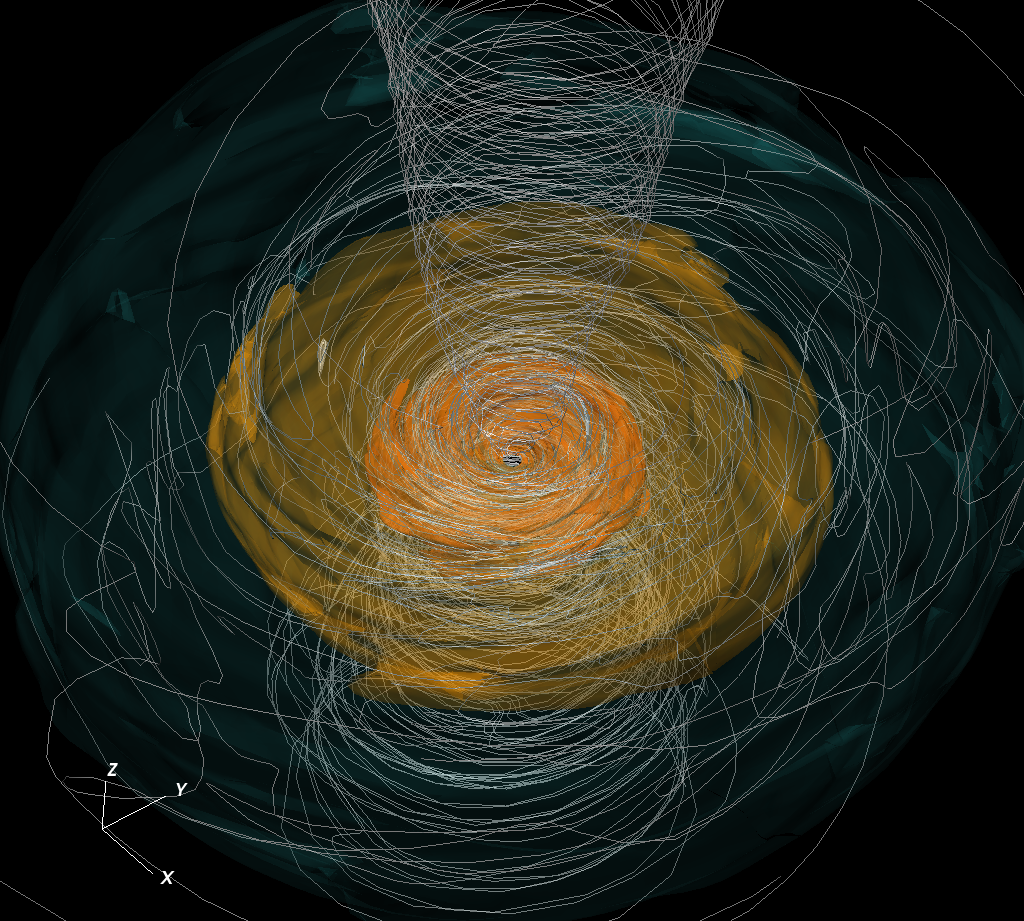
\includegraphics[width=0.45\textwidth]{figures/sane_3D.png}\hspace{1.5pt}%
  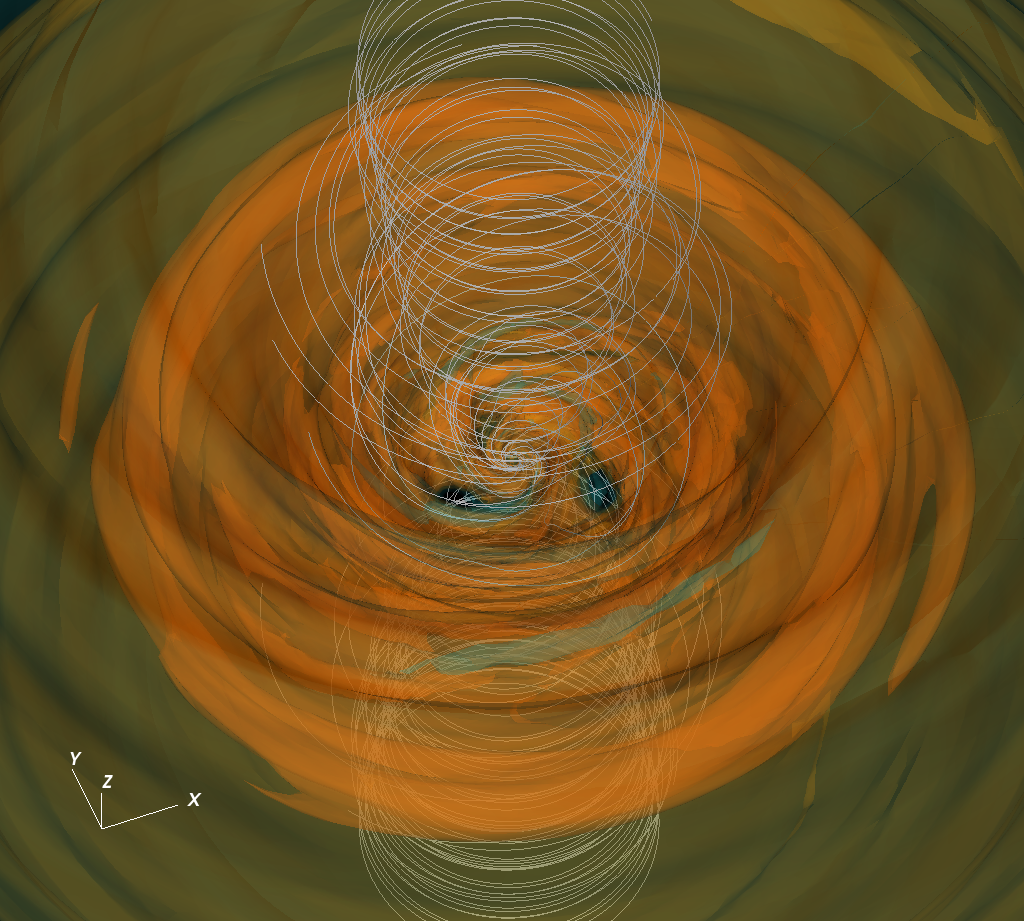
\includegraphics[width=0.45\textwidth]{figures/mad_3D_new.png}\\
  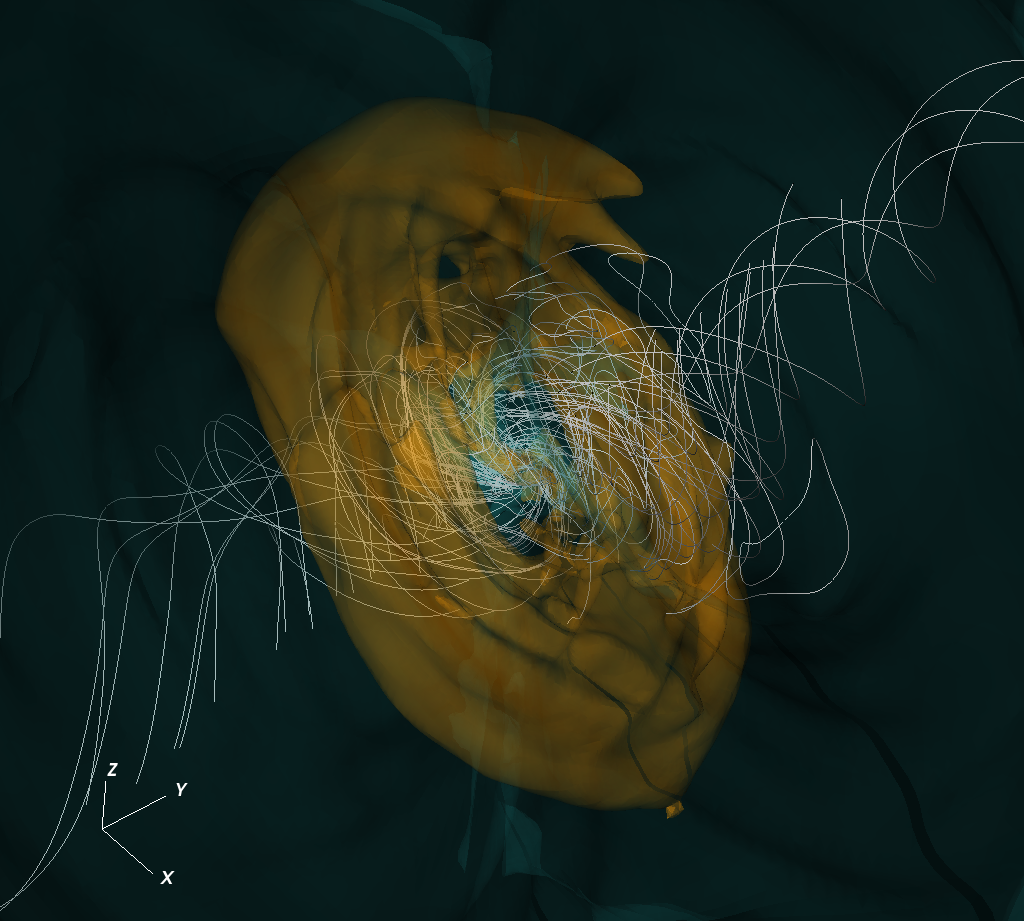
\includegraphics[width=0.45\textwidth]{figures/tilted_3D.png}\hspace{1.5pt}%
  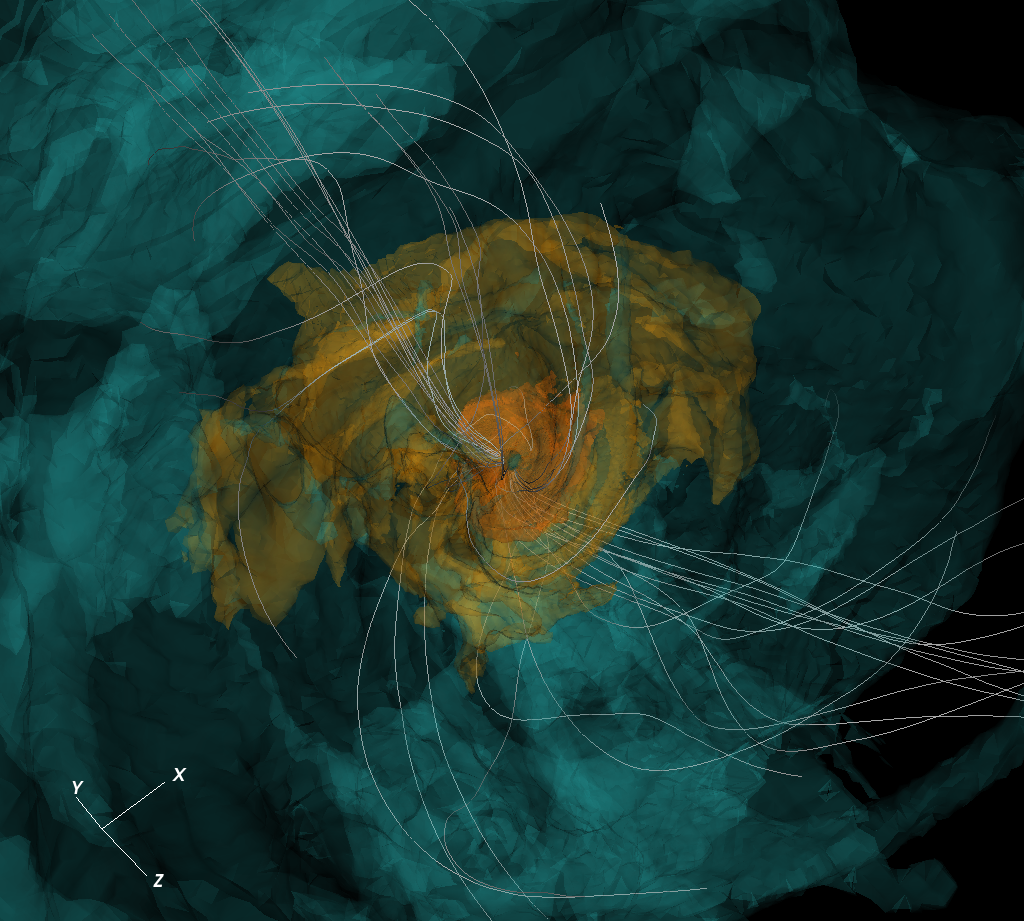
\includegraphics[width=0.45\textwidth]{figures/ressler_3D_new.png}
  \caption{3-D overview of selected GRMHD simulations of \sgra in our library. The color marks constant dimensionless density surfaces and lines follow magnetic field lines. Two top panels show standard accretion models: SANE (left panel, $a_*=+15/16$) and MAD (right panel, $a_*=0.5$). Two bottom panels show non-standard accretion models: tilted disk (left panel, $a_*=+15/16$ and titlt angle of 60 deg) and Wind Accretion (right panel, $a_*=0$). In case of spinning black holes, the spin is aligned with z-axis. \monika{plots are not final, more detailed quantitative plots of models are expected to be in the appendix.}
  \aeb{This looks great!}
  \gw{Presumably the MAD simulation ``only'' has field lines that thread the near-horizon region because the footpoints are distributed relative to field strength? Might be worthwhile to mention if so.}\monika{that is not the case. these images may change a bit in the near future}\gw{In that case, I definitely think we should explain how the magnetic field lines are chosen.} \aco{Monika, 3D rendering looks very nice. There are some way to choose same BH spin, view angle, limits on density and magnetic fields to see only differences in accretion models? } \ckc{If these are in normal spherical polar or cartesian, I suggest we also ask Matt Turk to try visualizing them yt.}\monika{thanks for all the suggestions, will incorporate before submission.}}
  \label{fig:GRMHD}
\end{figure*}

% \paragraph{Methods, initial and boundary conditions:}
We model the plasma flow around \sgra using ideal, non-radiative GRMHD.  The gravitational field is given by the Kerr metric, with mass given by Equation (\ref{eq:mass}) and with black hole spin $\abh$ as free parameter \citep[see e.g.,][]{2003ApJ...589..444G, 2005ApJ...635..723A, 2007A&A...473...11D}.

We integrate the GRMHD equations in three spatial dimensions using multiple methods: {KHARMA} \citep{2021JOSS....6.3336P}, BHAC \citep{2017ComAC...4....1P}, HAMR \citep{2018MNRAS.474L..81L}, Koral \citep{2013MNRAS.429.3533S} and Athena++ \citep{2016ApJS..225...22W}; see \citealt{2019ApJS..243...26P} and \citet[in prep]{Olivares_et_al} for a comparison of GRMHD codes.  All simulations assume a constant adiabatic index $\Gamma_{\rm ad}$.

The \emph{standard} initial conditions for the GRMHD integrations are a hydrodynamic, constant-angular-momentum equilibrium, the Fishbone-Moncrief torus \citep{1976ApJ...207..962F}\aco{\citep[see also][]{2002MNRAS.334..383F}}\monika{why do we need to have this second citation? is that essential?}\br{I thought Font shows another hydro torus equilibrium in this paper? We don't use that one, so I would not cite that paper} in a prograde ($\abh > 0$) or retrograde ($\abh < 0$) orbit.  In all models except the HAMR-Tilted models the torus orbital angular momentum is either parallel or antiparallel to the black hole spin. The torus is parametrized by an inner radius $R_{\rm in}$, typically $12\rg$, and the pressure maximum radius $R_{\rm max}$, typically $24\rg$.
The torus is seeded with a weak, poloidal magnetic field %\aco{ with magnetization $\beta \equiv p_{\rm gas}/p_{\rm mag} =100$}.
% we dont want to elaborate on details like that here

All simulations are run in horizon penetrating Kerr-Schild coordinates, which are regular on the horizon.  Most are run in a variant of spherical polar coordinates.  The {\em standard} boundary conditions are outflow at the inner boundary, located inside the event horizon, outflow at the outer boundary, located at $r \gtrsim 1000 \rg$, and reflecting boundary conditions at the poles.  Standard  simulations are evolved to $t_f=30,000 \tg$.

Once the evolution has started, a combination of instabilities including the magnetorotational instability (MRI, \citealt{1992ApJ...400..610B}) drives the torus to a turbulent, fluctuating state. The standard accretion flow models can be divided by  latitude into three zones: equatorial inflow, a mid-latitude disk wind (``corona''; $\beta \equiv p_{gas}/[B^2/(8\pi)] \sim 1$) and a polar relativistic jet (``funnel''; $\sigma \equiv B^2/(8\pi \rho c^2) \gtrsim 1$).

It is well established (see e.g., \citetalias{M87PaperV}, \citetalias{M87PaperVIII} and references therein) that the magnetic flux through the event horizon divides the outcomes into two categories: the Magnetically Arrested Disk (MAD) state \citep[e.g.,][]{1974Ap&SS..28...45B, Igumenschchev:2003, 2003PASJ...55L..69N} in which the magnetic flux near the horizon saturates and significantly affects the dynamics of the flow, and the Standard and Normal Evolution (SANE) state \citep[e.g.,][]{2003ApJ...589..444G, devilliers:2003, Narayan:2012}.  The relative importance of magnetic flux can be described by $\phi \equiv \Phi_{\mathrm{BH}} (\dot{M} r_g^2 c)^{-1/2}$, where $\Phi_{\rm BH}$ is the magnetic flux interior to the black hole equator and $\dot{M}$ is the mass accretion rate through the horizon. MAD models have $\phi \sim \phi_{crit} \sim 60$. \footnote{In the Lorentz-Heaviside units commonly used in GRMHD simulations $\phi_\mathrm{crit}$ is smaller by a factor of $(4\pi)^{1/2} \simeq 3.545$.} \aco{Should we cite the work-in-progress by Narayan about spinup-spindown for MAD models where magnetic flux it can be written as a function of BH spin? I've verified the same tendency for BHAC.}\monika{not necessary, this is not established and should be first published we want to limit in prep as much as possible} In MAD models magnetic flux accretes onto the hole until $\phi \gtrsim \phi_{crit}$, then magnetic flux is expelled from the hole and escapes through the inflowing plasma.  SANE models have $\phi < \phi_c$, and in most of our standard models have $\phi \sim 1$.

We also consider two \emph{non-standard} GRMHD simulations: strongly magnetized non-MAD tilted torus simulations \citep{Liska2018, Chatterjee2020} and a model in which \sgra is fed directly by winds from stars in its vicinity \citep{2020ApJ...896L...6R}. The self-consistent wind feeding simulations result in a mode of accretion that is somewhat similar to MAD but typically has lower mean angular momentum and is less well organized.
These wind-fed models have $\abh = 0$.

The GRMHD model library is summarized in Table~\ref{tab:GRMHDmodels}. In Figure~\ref{fig:GRMHD} we show a few examples of standard and non-standard GRMHD runs. The models vary in numerical method and in numerical resolution. We present more information on the numerical methods and models in Appendix~\ref{app:numerical} and in  Appendix~\ref{app:variability}.

%------------------------------------------------------------------------------
\subsubsection{Radiative Transfer Model}

Synthetic observations are generated from the GRMHD model in a radiative transfer step.
The transfer step requires: %(1) CK: I prefer using i), ii), iii) in text because (1) is used for equations.
\emph{i})~a model for the electron temperature and electron distribution function (hereafter eDF);
\emph{ii})~an assignment of a density scale to the GRMHD model;
\emph{iii})~a numerical radiative transfer step done after the GRMHD model, assuming that the plasma evolution is unaffected by radiation.

\subsubsubsection{Electron Distribution Function}

In {\it thermal} models electron energies are distributed into the Maxwell-J{\"u}ttner distribution function:
\begin{align}
\frac{1}{n_e}\frac{dn_e}{d\gamma}= \frac{\gamma^2 \sqrt{1-1/\gamma^2}} {\Theta_e K_2(1/\Theta_e)} \exp\left(-\frac{\gamma}{\Theta_e}\right);
\end{align}
recall $\Theta_e=k_b T_e/m_e c^2$, which is determined by the ion-electron temperature ratio $R \equiv T_i/T_e$:
\begin{align}
T_e=\frac{2 m_p u}{3 k_B \rho (2+R)}.
\end{align}
Here $u$ and $\rho$ are the internal energy density and rest-mass density from the GRMHD simulation.  Thermal models are motivated by the idea that wave-particle scattering drives partial relaxation of the eDF, even though Coulomb scattering is ineffective.

In \citetalias{M87PaperV} and \citetalias{M87PaperVIII}, $R$ is assigned using a prescription, adopted from \cite{2016A&A...586A..38M}, that assumes (1) the temperature ratio is a function only of local conditions (2) the ratio varies from one value at low plasma $\beta \equiv P_\mathrm{gas}/P_\mathrm{mag}$ to a second value at high $\beta$:
\begin{equation}
R = \frac{T_i}{T_e} = \Rh \frac{b^2}{b^2+1} + \Rl \frac{1}{b^2+1}.
\end{equation}
Here $b \equiv \beta/\beta_\mathrm{crit}$. This model has three free parameters: $\beta_\mathrm{crit}$, $\Rl$, $\Rh$.  In the standard models $\Rl = 1$, $\beta_\mathrm{crit} = 1$, and only $\Rh$ is allowed to vary from $1$ to $160$.  The $\Rh$ model is motivated by plasma heating models in which the branching ratio for dissipation into ions and electrons approaches $1$ at low $\beta$ \citep[e.g.,][]{2010MNRAS.409L.104H,Kawazura771}.

In {\it non-thermal} models the eDF includes a power-law tail extending to high energy.
%\jd{this needs some references to kappa-jet work. e.g. Davelaar+2018\&2019} % already cited earlier in text
This is implemented in two ways: with a so-called $\kappa$ distribution function, inspired by observations of the solar wind and by results of
collisionless plasma simulations (e.g., Kunz et al. 2015 and references therein):
%\jd{only solar wind? this looks not complete yet, Kunz+2015, and two papers on kappa-jet models that show that kappa-df models get the SED of SgrA*/M87 right...}
%Davelaar wonderful papers are already cited earlier
\begin{align}
  \frac{1}{n_e} \frac{d n_e}{d\gamma}= \gamma \sqrt{\gamma^2-1} \left(1+\frac{\gamma+1}{\kappa w}\right)^{-(\kappa+1)}
\end{align}
which has width parameter $w$ and power-law index parameter $\kappa$, or with a power-law distribution function:
\begin{align}
  \frac{d n_e}{d\gamma} =
  n_e \frac{ (p-1)}{({\gamma^{1-p_\mathrm{pl}}_\mathrm{min}} - {\gamma^{1-p}_\mathrm{max}})} \gamma^{-p_\mathrm{pl}}
  \label{eq:nonthermaleDF}
\end{align}
which has power-law index $p_{pl}$ and upper and lower limits  $\gamma_{\min}$ and $\gamma_{\max}$.

Evidently any eDF assignment schemes is an approximation in the sense that the eDF will in general depend on both local conditions and particle histories.  The eDF is assumed isotropic, and electron-positron pairs are neglected (refs!).

Once the eDF is specified the radiative transfer coefficients (emissivities, absorptivities, and rotativities) can be readily calculated; see \cite{2021ApJ...921...17M} for a recent summary.

%\kc{Perhaps add a plot of the different eDFs to display the variety of models considered.}

%..............................................................................
\subsubsubsection{Model Scaling}

With the exception of the special stellar wind-fed simulations, the GRMHD models considered in this work are scale-free.  Physical units are assigned during the radiative transfer step.  The black hole mass $\mbh$ fixes the length unit $\rg$ and time unit $\tg$.  The GRMHD models are not self-gravitating, however, and therefore one is free to set a density scale, or equivalently the accretion rate $\dot{M}$ or mass unit $\Munit$.

The density in cgs units ($\rho_\mathrm{cgs}$) is obtained from the density  in simulation units ($\rho_\mathrm{sim}$) via $\rho_\mathrm{cgs} = \rho_\mathrm{sim} \Munit_\mathrm{cgs} {(\rg)}_\mathrm{cgs}^{-3}$.  Similarly, $u_\mathrm{cgs} = u_\mathrm{sim} \Munit_\mathrm{cgs} {(\rg)}_\mathrm{cgs}^{-3} c_\mathrm{cgs}^2$, and $B_\mathrm{cgs} = (4\pi)^{1/2} B_\mathrm{sim} \Munit_\mathrm{cgs}^{1/2} {\rg}_\mathrm{cgs}^{-3/2} c_\mathrm{cgs}$; the factor of $(4\pi)^{1/2}$ comes from converting Heaviside-Lorentz units (used in GRMHD simulations) to cgs.
The simulation density scale $\Munit$ is a free parameter.  It is fixed through an iterative process so that the mean $230$GHz flux density of the model matches the $\simeq 2.4$~Jy observed mean from the 2017 campaign (see next section).

%..............................................................................
\subsubsubsection{Radiative Transfer Calculation}

Given an eDF, density scale $\Munit$, and radiative transfer coefficients, the emergent radiation is obtained by solution of the radiative transfer equation.  For this we use two classes of numerical methods: ray tracing to generate synthetic images, and a Monte Carlo scheme to generate spectral energy distributions (SEDs).  Further detail on numerical methods is given Appendix \ref{app:radtrans}.  Comparisons of numerical methods \citep[][Prather et al. 2021]{2020ApJ...897..148G} shows that differences between numerical schemes do not contribute significantly to the error budget.

The models are imaged at $86$GHz, $230$~GHz~\footnote{The mean frequency for  EHT observations is more nearly $228$~GHz.} and $2.2\mu$m.  Direct imaging includes synchrotron emission and absorption and bremsstrahlung (both ion-electron and electron-electron; see \citet{2020ApJ...898...50Y} for a recent review).  The SED is averaged over a narrow range in inclination and over all position angles. The SED includes synchrotron, bremsstrahlung, {\em and} Compton scattering.  NIR emission is usually dominated by synchrotron, but we find that occasionally NIR synchrotron is so weak that Compton scattering dominates.  The X-ray is dominated by bremsstrahlung or Compton scattering.
In Figure~\ref{fig:fiducial_imgs} we present a few examples of time-averaged model images and multiwavelenght SEDs of selected standard \sgra models.

%==============================================================================
\subsection{Summary of Sgr~A* model library}

A summary of all radiative transfer calculations is given in Table~\ref{tab:radiativemodels}.
\note{Entire image library contains $MMM$ model sets, $NNN$ models, $PPP$ images, and $QQQ$ SEDs and occupies $GGG$ gigabytes.}

\begin{figure*}
  \centering
  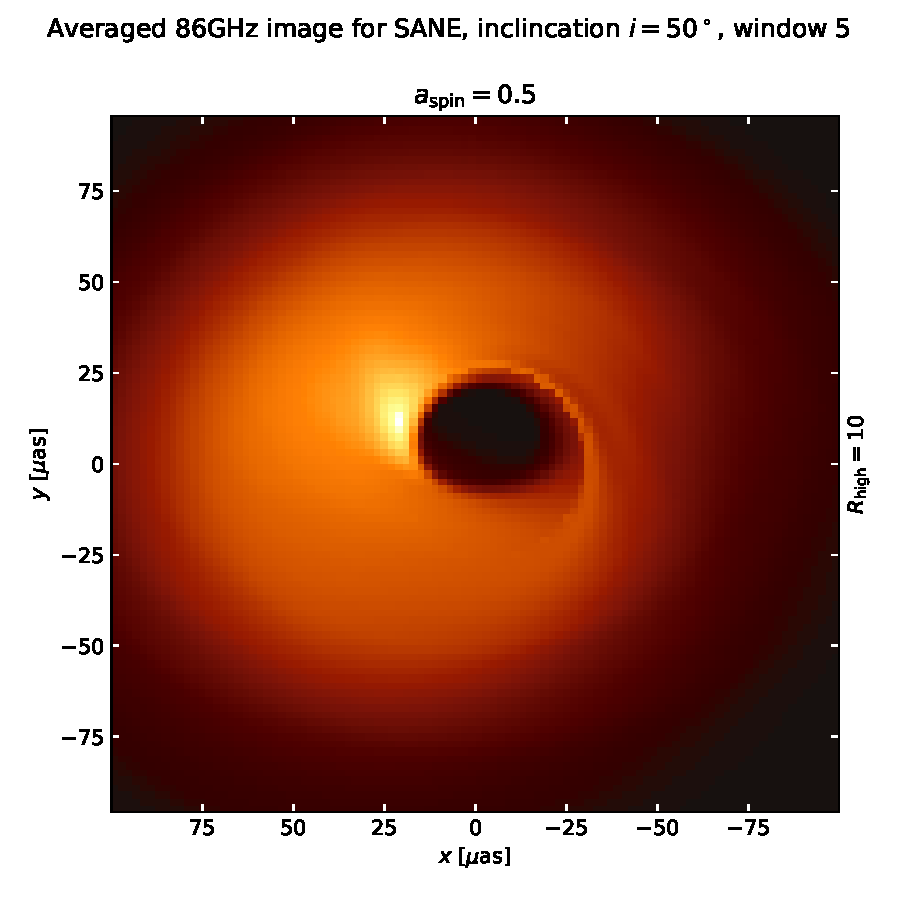
\includegraphics[width=0.333\textwidth]{figures/avgsample_SANE_86GHz.pdf}%
  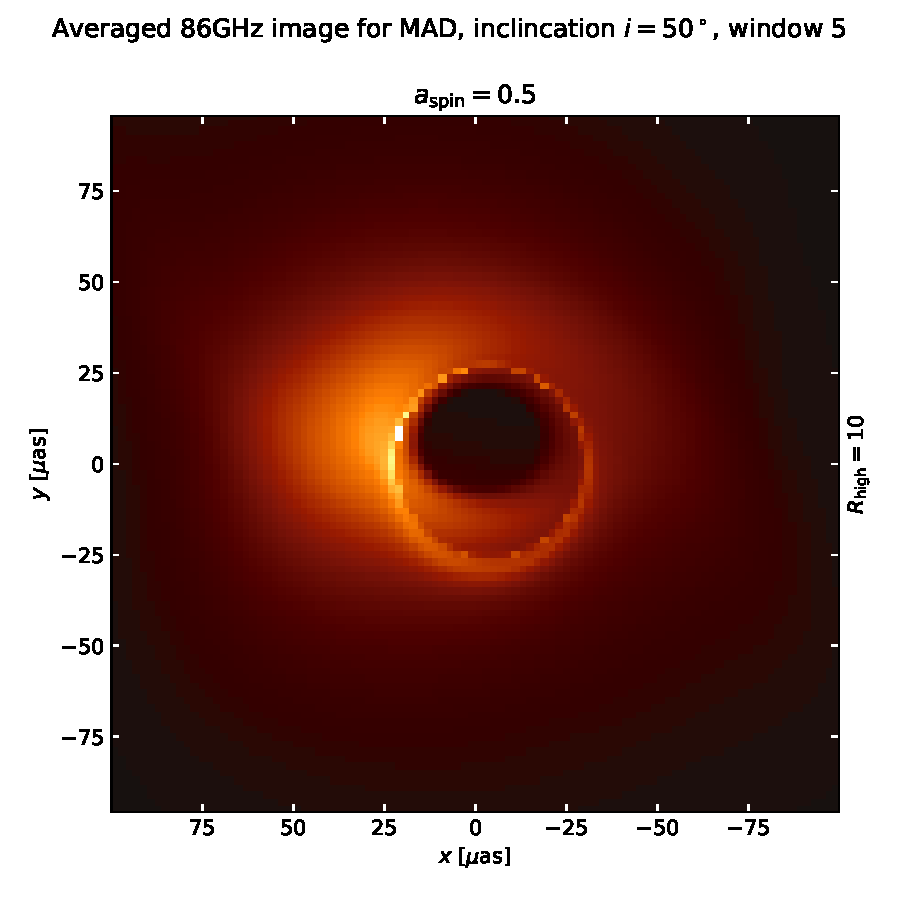
\includegraphics[width=0.333\textwidth]{figures/avgsample_MAD_86GHz.pdf}%
  \includegraphics[width=0.333\textwidth]{figures/avgsample_kappa_86GHz.pdf}\\
  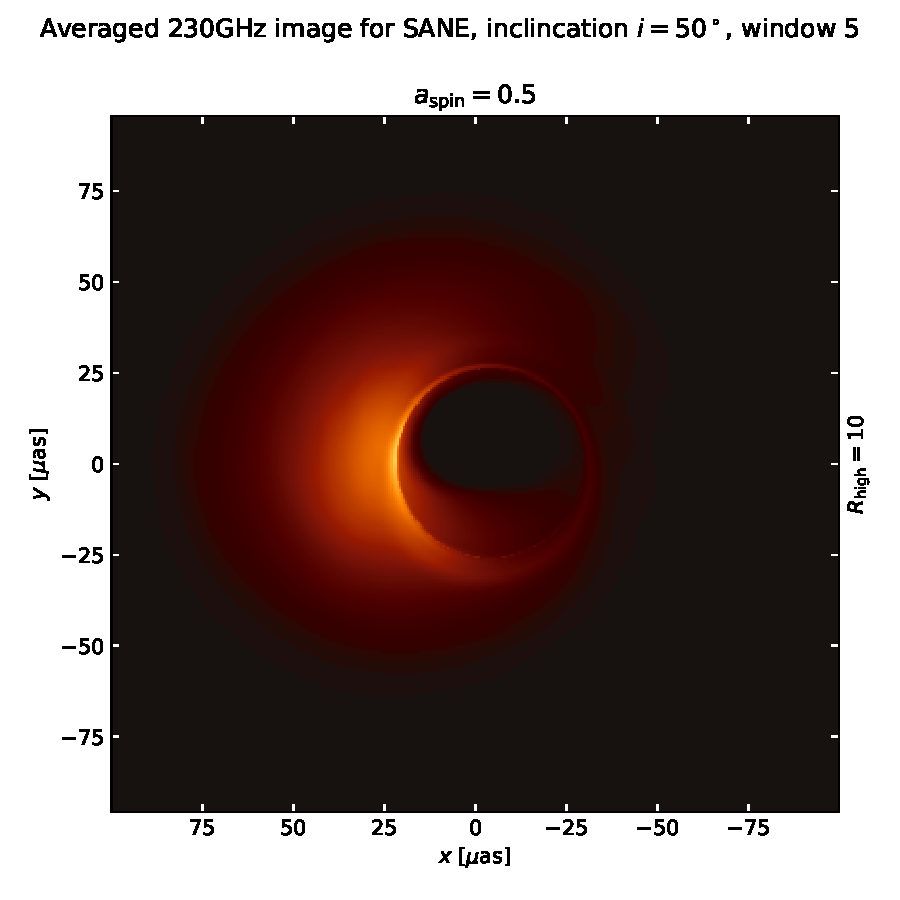
\includegraphics[width=0.333\textwidth]{figures/avgsample_SANE.pdf}%
  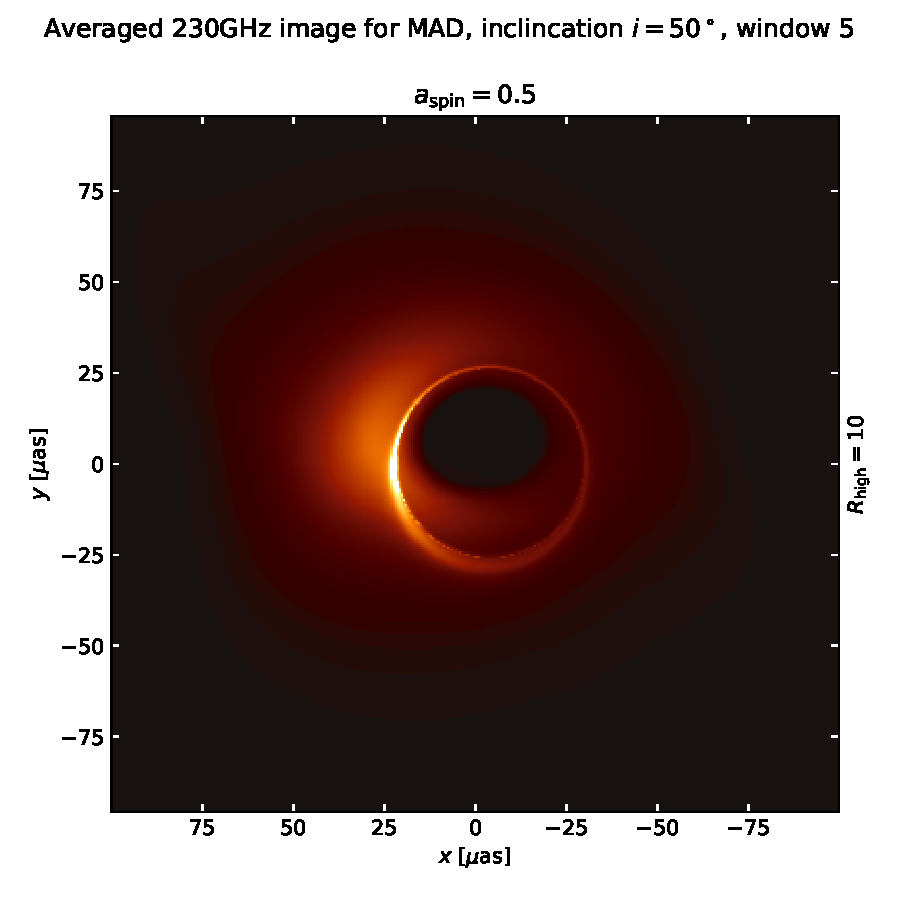
\includegraphics[width=0.333\textwidth]{figures/avgsample_MAD.pdf}%
  \includegraphics[width=0.333\textwidth]{figures/avgsample_kappa.pdf}\\
  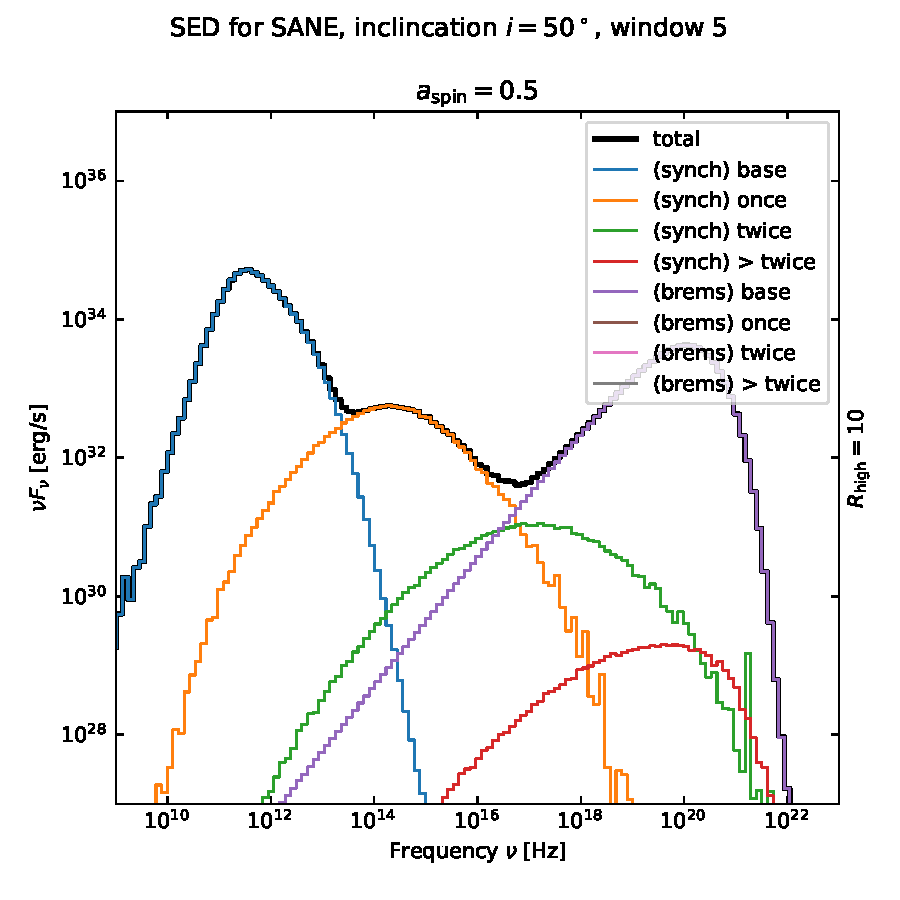
\includegraphics[width=0.333\textwidth]{figures/sedsample_SANE.pdf}%
  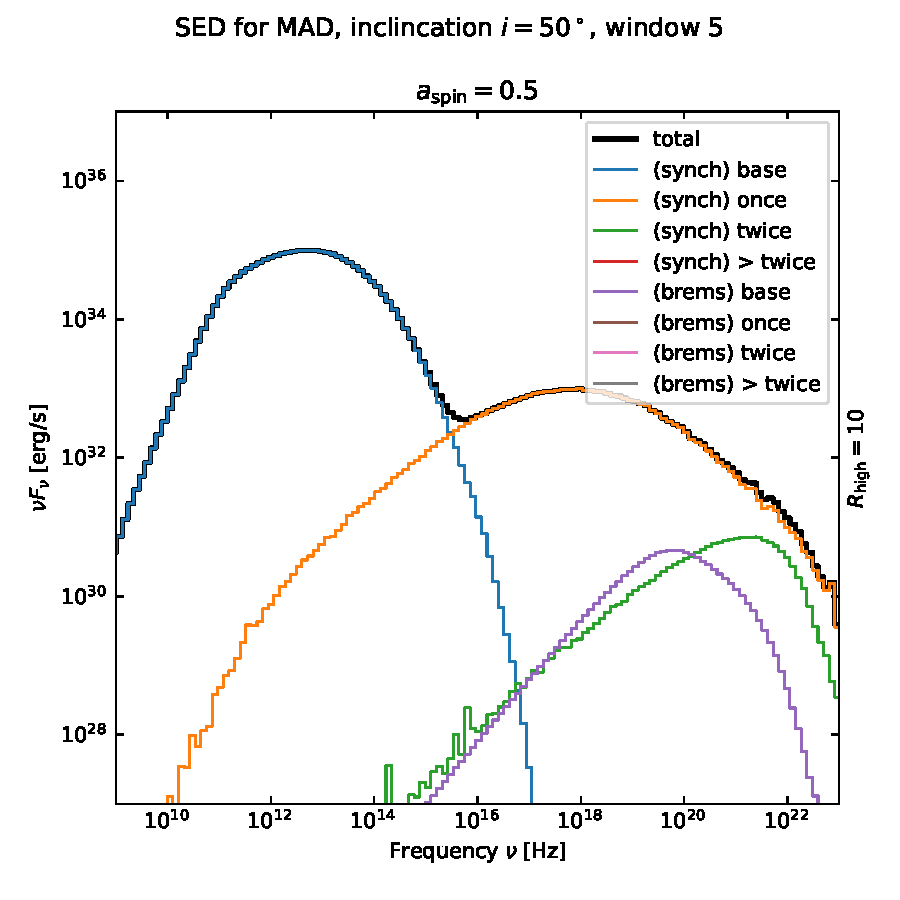
\includegraphics[width=0.333\textwidth]{figures/sedsample_MAD.pdf}%
  \includegraphics[width=0.333\textwidth]{figures/sedsample_kappa.pdf}
  \caption{Time-averaged images and corresponding time-averaged SEDs from the simulation library:
    (a) thermal SANE, (b) thermal MAD, and (c) non-thermal SANE.\monika{labels have to be made larger}\ckc{will do.  86GHz currently uses lower resolution.  We can either interpolate, or increase the resolution for these fudicial models.}\monika{I suggest to make big white labels on images with frequency and viewing angle and model type, window time we can give in figure caption. SEDs could have small arrows pointing at which frequency in the SED the images are made demonstraitng that we see only synchrotron emission at 86 and 230 GHz (and no e.g. bremsstrahlung), spins could be also mentioned in figure caption.}}
  \label{fig:fiducial_imgs}
\end{figure*}

%\clearpage
%\pagebreak
%\movetabledown=3cm % recommended in AASTeX docs to center table on page
%\begin{rotatetable}
\begin{deluxetable*}{ccccccccccc}
\tabletypesize{\footnotesize}
\renewcommand{\arraystretch}{1.1}
\tablehead{
  \colhead{Model} &%
  \colhead{$\Rl$}                  &%
  \colhead{$\Rh$}                  &%
  \colhead{$\beta_{\rm crit}$}     &%
  \colhead{$p_{pl}$}                    &%
 %% \colhead{$\gamma_{\rm min/max}$} &%
  \colhead{$\kappa$}               &%
  \colhead{$i^\circ$}              &%
  \colhead{$\nu$}             &%
  \colhead{SED}                    &%
  \colhead{$\Delta t$}    &%
  \colhead{\#frames_{230}}       \\
 &  & & & & & & \colhead{[GHz]} & & \colhead{[1000 M]} &
    }
\startdata
\multicolumn{11}{c}{\bf Thermal models}\\
KHARMA & 1 & [1,10,40,160] & 1 & - & - & [10,30,...,170] & [86,230] & Yes & [15,20) &  $360,000$ \\
KHARMA & 1 & [1,10,40,160] & 1 & - &  - & [10,30,...,170] & [86,230] & Yes & [20-25) & $360,000$ \\
KHARMA & 1 & [1,10,40,160] & 1 & - &  - & [10,30,...,170] & [86,230] & Yes & [25-30) & $360,000$\\
BHAC & 1 & [1,10,40,160] & 1 & - &  - & [10,30,...,90]  & [86,230] & Yes & [10-15) & $100,000$ \\
BHAC & 1 & [1,10,40,160] & 1 & - &  - & [10,30,...,90]  & [86,230] & Yes & [20-25) & $100,000$ \\
BHAC & 1 & [1,10,40,160] & 1 & - &  - & [10,30,...,90]  & [86,230] & Yes & [25-30) & $100,000$ \\
HAMR & 1 & [1,40,160] & 1 & - & - &  [10,50,90]  & [86,230] & Yes & [30-35) & x \\
KORAL& 1 & [?]    & 1 & - & - &  [10,30,...,90]      & [86,230]  & ?   & ?       & x \\
Wind Accretion& 1 & [?]    & 1 & - & - &  [10,30,...,90]      & [86,230]  & ?   & ?       & x \\
HAMR Tilted & 1 & [1,40,160] & 1 & - & - &  [10,50,90]  & [86,230] & Yes & [100-103) & x \\
\hline
\multicolumn{11}{c}{\bf Thermal + non-thermal power-law models}\\
HAMR & 1 & [1,40,160] & 1 & 4 & - &  [10,50,90]  & [86,230] & No & [30-35) & x \\
\hline
\multicolumn{11}{c}{\bf Thermal + non-thermal $\kappa$ models}\\
BHAC & 1 & [1,10,40,160]  & 1 & -  &  3.5 ($\epsilon_0=0.05$) & [10,30,...,90]  & [86,230] & No & [25-30) & 20,000  \\
BHAC & 1 & [1,10,40,160]  & 1 & -  &  3.5 ($\epsilon_0=0.10$) & [10,30,...,90]  & [86,230] & No & [25-30) & 20,000  \\
BHAC & 1 & [1,10,40,160]  & 1 & -  &  3.5 ($\epsilon_0=0.20$) & [10,30,...,90]  & [86,230] & No & [25-30) & 20,000 \\
BHAC & 1 & [1,10,40,80,160]  & 1 & -  &  variable $\kappa=\kappa(\beta,\sigma)$  & [10,30,...,90]  & [86,230] & No & [25-30) & $125,000$ \\
HAMR & 1 & [1,10,40,160] & 1 & - &  variable $\kappa=\kappa(\beta,\sigma)$ & [10,30,...,90]  & [86,230] & Yes & [25-30) & $100,000$ \\
\enddata
\caption{Summary of emission simulations in \sgra EHT model library.\kc{flipped PL and kappa, and propose to remove $\gamma_{\rm min/max}$ from the table as it is a local quantity in hamr models} The cadence of KHARMA=5M, BHAC=10M for thermal and nonthermal variable kappa, 50M for nonthermal variable efficiency models. variable kappa HAMR cadence is 10M.
\gw{Rhigh for the wind accretion models is either 28 or 13, but these are for two separate simulations (so it's not like there's one simulation where Rhigh has been varied)}
}~\label{tab:radiativemodels}
\end{deluxetable*}
%\end{rotatetable}

%\pagebreak
%\clearpage
% %..............................................................................
% \subsubsection{Thermal Models}
%
% ...
%
% \paragraph{Illinois Models}
%
% % Please fill in basic information of the models in the following list.
% % Please add more details if necessary. A full paragraph description
% % of the model is welcome, but not required at this point.
% \begin{itemize}[noitemsep]
% \item $a_\mathrm{spin}$: 0, $\pm1/2$, $\pm15/16$
% \item Magnetic Flux: MAD, SANE
% \item Adiabatic Index $\Gamma$: 4/3
% \item Time $t_\mathrm{final}$: 30,000$M$
% \item $\rho_0$: 3 different density normalization chosen for each parameter set for $t \in [15,000, 20,000), [20,000, 25,000), [25,000, 30,000)$.
% \item $\Rh$: 1, 10, 40, 160
% \item Inclination $i$: 10$^\circ$, 30$^\circ$, 50$^\circ$, ..., 170$^\circ$
% \item Resolution:
% \item Initial conditions:
% \item Reference: this work
% \item Status: w4 and w5 all done; w3 in progress
% \end{itemize}
%
% \paragraph{Frankfurt Models}
%
% % Please fill in basic information of the models in the following list.
% % Please add more details if necessary. A full paragraph description
% % of the model is welcome, but not required at this point.
% \begin{itemize}[noitemsep]
% \item $a_\mathrm{spin}$: 0, $\pm1/2$, $\pm15/16$
% \item Magnetic Flux: MAD, SANE
% \item Adiabatic Index $\Gamma$: 4/3
% \item Time $t_\mathrm{final}$: 30000
% \item $\rho_0$: 3 different density normalizations chosen for each parameter set for $t \in [10,000, 15,000), [20,000, 25,000), [25,000, 30,000)$
% \item $\Rh$: 1, 2.5, 5, 10, 40, 160
% \item Inclination $i$: 10$^\circ$, 30$^\circ$, 50$^\circ$,..., 90$^\circ$
% \item Resolution:
% \item Initial conditions:
% \item Reference: this work
% \item Status: all done except for SANE a=-15o16
% \end{itemize}
%
% \paragraph{HAMR Models}
%
% % Please fill in basic information of the models in the following list.
% % Please add more details if necessary. A full paragraph description
% % of the model is welcome, but not required at this point.
% \begin{itemize}[noitemsep]
% \item $a_\mathrm{spin}$: 0, $\pm1/2$, $\pm15/16$
% \item Magnetic Flux: MAD, SANE
% \item Adiabatic Index $\Gamma$: 13/9, 5/3
% \item Time $t_\mathrm{final}$: $35,000M$
% \item $\rho_0$: 1 density normalization for $[30,000-35,000)M$
% \item $\Rh$: 1, 40, 160
% \item Inclination $i$: 10$^\circ$, 50$^\circ$, 90$^\circ$
% \item Resolution: $348\times 192\times 192$, $240\times 192\times 192$
% \item Initial conditions: FM: $r_{\rm in}=6, 20M$; $r_{\rm pmax}=12, 41M$
% \item Grid outer radius: $1000M$, $200M$
% \item Reference: this work
% \item Status: GRMHD simulations done
% \end{itemize}
%
% %..............................................................................
% \subsubsection{Non-thermal (power-law )Models}
%
% ...
%
% \paragraph{Frankfurt Models}
%
% % Please fill in basic information of the models in the following list.
% % Please add more details if necessary. A full paragraph description
% % of the model is welcome, but not required at this point.
% \begin{itemize}[noitemsep]
% \item $a_\mathrm{spin}$: 0, $\pm1/2$, $\pm15/16$
% \item Magnetic Flux: MAD, SANE
% \item Adiabatic Index $\Gamma$:
% \item Time $t_\mathrm{final}$:
% \item $\rho_0$:
% \item Power law fraction $f$:
% \item Power law index $p$:
% \item Inclination $i$:
% \item Reference:
% \item Status: no power-law model so far
% \end{itemize}

% \paragraph{HAMR Models}

% % Please fill in basic information of the models in the following list.
% % Please add more details if necessary. A full paragraph description
% % of the model is welcome, but not required at this point.
% \begin{itemize}[noitemsep]
% \item $a_\mathrm{spin}$: 0, $\pm1/2$, $\pm15/16$
% \item Magnetic Flux: MAD, SANE
% \item Adiabatic Index $\Gamma$: 13/9, 5/3
% \item Time $t_\mathrm{final}$: $35,000M$
% \item $\rho_0$: 1 density normalization for $[30,000-35,000)M$
% \item $\Rh$: 1, 40, 160
% \item Inclination $i$: 10$^\circ$, 50$^\circ$, 90$^\circ$
% \item Resolution: $348\times 192\times 192$, $240\times 192\times 192$
% \item Initial conditions: FM: $r_{\rm in}=6, 20M$; $r_{\rm pmax}=12, 41M$
% \item Grid outer radius: $1000M$, $200M$
% \item Reference: this work
% \item Status: GRMHD simulations same as for thermal models
% \end{itemize}
%
% %..............................................................................
% \subsubsection{Non-thermal ($\kappa$) Models}
%
% ...
%
% % Please fill in basic information of the models in the following list.
% % Please add more details if necessary. A full paragraph description
% % of the model is welcome, but not required at this point.
% \begin{itemize}[noitemsep]
% \item $a_\mathrm{spin}$: 0, $\pm1/2$, $\pm15/16$
% \item Magnetic Flux: MAD, SANE
% \item Adiabatic Index $\Gamma$:
% \item Time $t_\mathrm{final}$:
% \item $\rho_0$:
% \item $\kappa$:
% \item Inclination $i$:
% \item Reference:
% \item Status:
% \end{itemize}
%
% \paragraph{Frankfurt Models}
%
% % Please fill in basic information of the models in the following list.
% % Please add more details if necessary. A full paragraph description
% % of the model is welcome, but not required at this point.
% \begin{itemize}[noitemsep]
% \item $a_\mathrm{spin}$: 0, $\pm1/2$, $\pm15/16$
% \item Magnetic Flux: MAD, SANE
% \item Adiabatic Index $\Gamma$: 4/3
% \item Time $t_\mathrm{final}$: 30000
% \item $\rho_0$: individual normalisation for each kappa model; only  for $t \in [25,000, 30,000)$
% \item $\kappa$: variable $\kappa(\beta, \sigma)$, fixed $\kappa=3.5$ with $\epsilon=\epsilon_{0} f(\beta,\sigma)$ for $\epsilon_{0}=0.05,0.10,0.20$
% \item $\Rh$: 1, 2.5, 5, 10, 40, 160
% \item Inclination $i$: 10$^\circ$, 30$^\circ$, 50$^\circ$,..., 90$^\circ$
% \item Reference: this work
% \item Status: in production
% \end{itemize}
%
% \paragraph{HAMR Models}
%
% % Please fill in basic information of the models in the following list.
% % Please add more details if necessary. A full paragraph description
% % of the model is welcome, but not required at this point.
% \begin{itemize}[noitemsep]
% \item $a_\mathrm{spin}$: 0, $\pm1/2$, $\pm15/16$
% \item Magnetic Flux: MAD, SANE
% \item Adiabatic Index $\Gamma$: 13/9, 5/3
% \item Time $t_\mathrm{final}$: $35,000M$
% \item $\rho_0$: 1 density normalization for $[30,000-35,000)M$
% \item $\kappa$: variable $\kappa (\beta, \sigma)$
% \item $\Rh$: 1, 40, 160
% \item Inclination $i$: 10$^\circ$, 50$^\circ$, 90$^\circ$
% \item Resolution: $348\times 192\times 192$, $240\times 192\times 192$
% \item Initial conditions: FM: $r_{\rm in}=6, 20M$; $r_{\rm pmax}=12, 41M$
% \item Grid outer radius: $1000M$, $200M$
% \item Reference: this work
% \item Status:
% \end{itemize}
%
% %..............................................................................
% \subsubsection{Critical $\beta$ Models}
%
% % Please fill in basic information of the models in the following list.
% % Please add more details if necessary. A full paragraph description
% % of the model is welcome, but not required at this point.
% \begin{itemize}[noitemsep]
% \item $a_\mathrm{spin}$:
% \item Magnetic Flux: MAD, SANE
% \item Adiabatic Index $\Gamma$:
% \item Time $t_\mathrm{final}$:
% \item $\rho_0$:
% \item Power law fraction $f$:
% \item Power law index $p$:
% \item Inclination $i$:
% \item Reference:
% \item Status:
% \end{itemize}
%
% %..............................................................................
% \subsubsection{Stellar Wind Accretion Models}
%
% % Please fill in basic information of the models in the following list.
% % Please add more details if necessary. A full paragraph description
% % of the model is welcome, but not required at this point.
% \begin{itemize}[noitemsep]
% \item $a_\mathrm{spin}$: 0
% \item Magnetic Flux: MAD, SANE
% \item Adiabatic Index $\Gamma$:
% \item Time $t_\mathrm{final}$:
% \item $\rho_0$:
% \item Power law fraction $f$:
% \item Power law index $p$:
% \item Inclination $i$:
% \item Reference:
% \item Status:
% \end{itemize}
%
% %..............................................................................
% \subsubsection{Koral Long MAD Models}
%
% % Please fill in basic information of the models in the following list.
% % Please add more details if necessary. A full paragraph description
% % of the model is welcome, but not required at this point.
% \begin{itemize}[noitemsep]
% \item $a_\mathrm{spin}$: 0, $\pm0.3$, $\pm0.5$, $\pm0.7$, $\pm0.9$
% \item Magnetic Flux: MAD
% \item Adiabatic Index $\Gamma$:
% \item Time $t_\mathrm{final}$: 100,000$M$
% \item $\rho_0$:
% \item Power law fraction $f$:
% \item Power law index $p$:
% \item Inclination $i$:
% \item Reference:
% \item Status:
% \end{itemize}
%
% %..............................................................................
% \subsubsection{Tilted Models}
%
% % Please fill in basic information of the models in the following list.
% % Please add more details if necessary. A full paragraph description
% % of the model is welcome, but not required at this point.
% \begin{itemize}[noitemsep]
% \item $a_\mathrm{spin}$: $+15/16$
% \item Magnetic Flux: INSANE
% \item Adiabatic Index $\Gamma$: 5/3
% \item Time $t_\mathrm{final}$: $>100,000M$
% \item $\rho_0$: 1 density normalization for $[100,000-103,000)M$
% \item $\Rh$: 1, 40, 160
% \item Inclination $i$: 10$^\circ$, 50$^\circ$, 90$^\circ$
% \item Resolution: $448\times 144\times 240$,
% \item Initial conditions: FM: $r_{\rm in}=12.5M$; $r_{\rm pmax}=25M$
% \item Grid outer radius: $100,000M$
% \item Reference: Chatterjee+20, Liska+18
% \end{itemize}
